\chapter{序論}


\section{研究背景}
\subsection{量子コンピューターの課題}
近年、量子コンピューターが話題に上がることが多くなってきた。
量子コンピューターは超並列計算機とも呼ばれ、因数分解、最適化計算に優れるため、同時に話題になっているAI(ディープラーニング)やビックデータなどとの相性が良いことがその一因であることが考えられる。既に商用化された量子コンピュータもあるが、まだまだ課題は多い。
量子コンピューターの動作原理である量子ビットには量子性を保ち制御できる仕組みが必要だが、現在それができる仕組みは多くなく、実用化に至るには様々な制約がある。
その中で、最も有力だと言われているものが「超伝導回路」による量子ビットである。
超伝導回路ではジョセフソン接合を用いて量子もつれ状態を実現しているが、
情報の保存時間であるコヒーレンス時間が現在数十マイク秒程度であり、
極低温下でしか動作しないなどの課題も多い。
北野研究室では、その課題解決に向けて高温超伝導体の固有ジョセフソン接合
(IJJ:Intrinsic Josephson Junction)を用いた超伝導量子ビットの実現を目指している。

\subsection{ジョセフソン接合}
二つの超伝導体が弱く結合した接合をジョセフソン接合と呼ぶ。
超伝導状態では、2つの電子が引力相互作用によりクーパー対を形成し、そのクーパー対の状態が巨視的な数重ね合わさり、一つの状態で記述することができるようになる。
この状態を記述する関数を、巨視的波動関数と呼ぶ。
ジョセフソン接合では2つの(巨視的波動関数の位相が)異なった超伝導体間に薄い絶縁体を挟むなどして弱く結合することにより、その2つの接合にトンネル電流が流れるという現象が見られる。

以下に模式図を示す。
\vspace{10 mm}

\begin{figure}[h]
  \begin{center}
    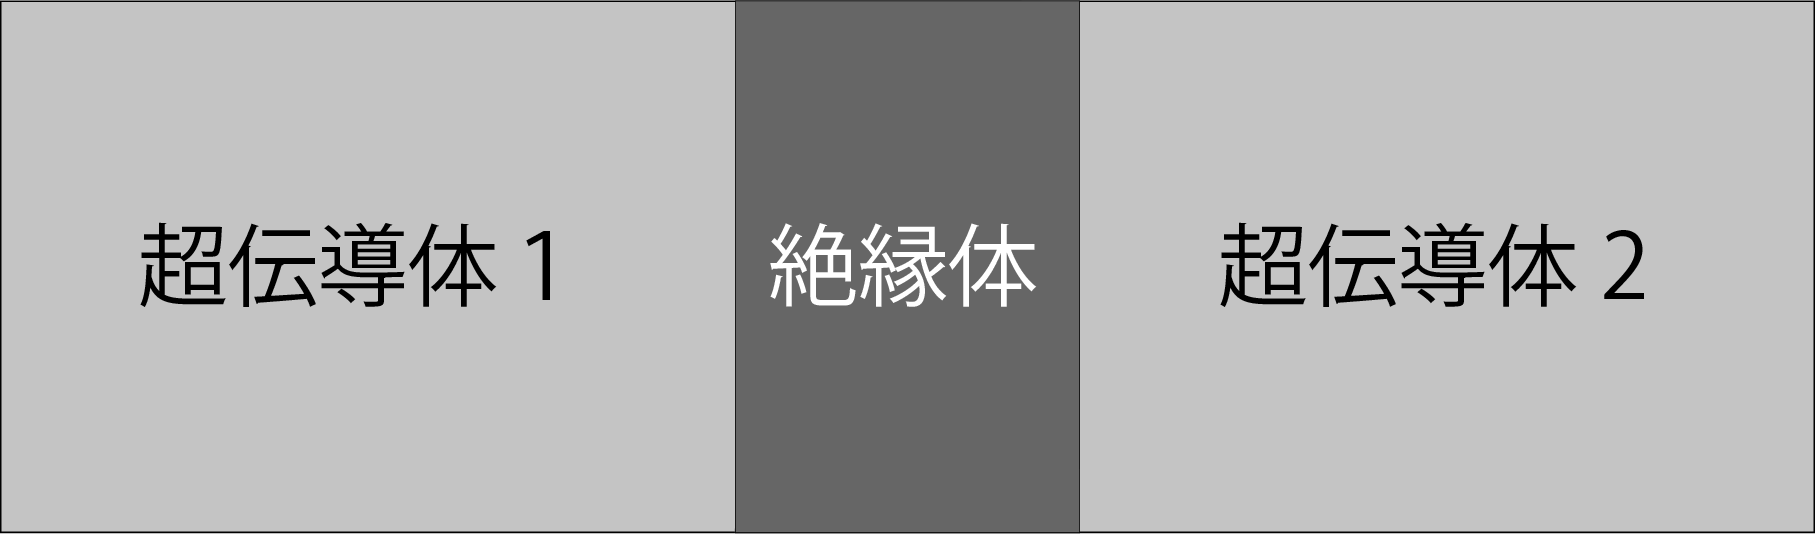
\includegraphics[width=5cm]{./image/JJ.png}
    \caption{ジョセフソン接合の模式図}
    \label{fig:JJ}
  \end{center}
\end{figure}
2つの超伝導体の位相差を$ \Delta \theta $とすると、そこに流れる超伝導電流は以下のように記述できる。

\[ I = I_c \sin{\Delta \theta } \]

\subsection{固有ジョセフソン接合}
超伝導体となる物質の中には、その物質の内部に絶縁体と超伝導が非常に薄い層状に重なっている構造をもつものが存在する。
そのような物質はその層間にジョセフソン接合があると視做すことができる。これを固有ジョセフソン接合と呼ぶ。

以下にその例として、Bi2212の構造を示す。\cite{びすます}
\vspace{10 mm}

\begin{figure}[h]
  \begin{center}
    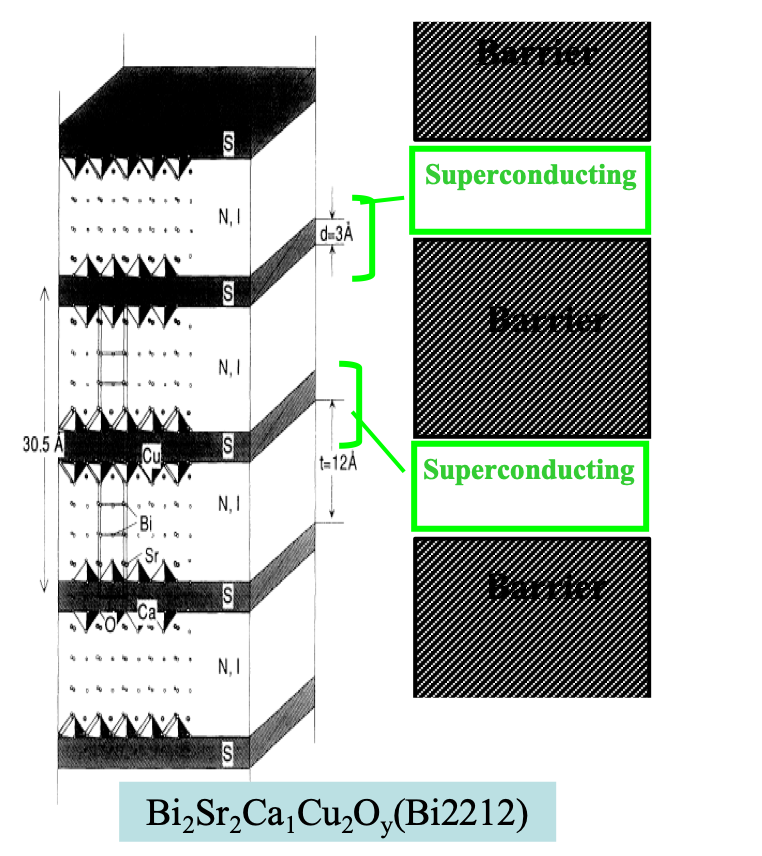
\includegraphics[width=5cm]{./image/IJJ.png}
    \caption{Bi2212の層状構造}
    \label{fig:Cavity}
  \end{center}
\end{figure}

北野研究室では、前述したような固有接合の研究を行っており、一例として、本研究室の修士課程を卒業された高橋優作氏の研究\cite{たかはし}では、Bi2212という超伝導体の固有ジョセフソン接合素子に41.5GHzのマイクロ波を照射した際にスイッチング確率の2重ピーク構造が観測された。このことからこの素子には離散化準位の形成があることが示された。
このほかにも、北野研の過去の研究では40GHz程度の周波数のマイクロ波で、同様の離散化順位の形成が観測された。

しかしこの固有ジョセフソン接合素子は、人口的に作成したジョセフソン素子とは異なり、実際に作成するまでどの程度のマイクロ波を照射すると離散化順位が形成されるのかがわからない。
素子の作成方法を工夫して、エネルギー順位を調整することは大変困難であるため、素子作成後にどの程度のエネルギー準位を有しているか調べるための方法が必要である。
今回は空洞共振器を用いてその準位を調べることを目指す。

\section{予備知識}
\subsection{マイクロ波空洞共振器}
マイクロ波とは周波数が数GHzから数十GHzほどの領域にある電磁波で、波長が電波より短く、遠赤外線より長い領域にある電磁波である。

一般に、高周波電流の流れている導体の周囲には電流を囲む円周方向に磁界$H$、あるいは磁束密度$B =μH$($μ$は媒質の透磁率)の磁束が生じる。
これは電磁気学におけるアンペールの法則として知られている現象である。
この磁束は、電流の周波数によって変化するため、ファラデーの電磁誘導則より、磁束に垂直な方向に電界E、あるいは電束密度$D =εE$(ここで$ε$は媒質の誘電率)で与えられる時間的に変化する電束が生じる。
このような電束の変化はそこに電流が流れていると同等に考えてよいため、再び新たな磁界が発生する。このようにして、伝搬していく波を電磁波と呼んでいる。電磁波は真空中でも伝搬する。

ある形状の管の中に音波を伝播させると特定の周波数で大きな音がなる現象は共振現象と呼ばれ、
管楽器など身近なところにも応用されている馴染みの深い現象であるが、
マイクロ波でも同様な現象が起こる。

一般に金完全導体で閉じられた中空の箱にマイクロ波を照射すると、
電磁場エネルギーが箱の中に蓄えられ、特定の周波数で電磁界振幅が増大する共振現象が起きる。
この中空の箱のことを空洞共振器と呼び、共振したときの周波数を共振周波数と呼ぶ。
一般に空洞共振器の共振周波数は、マクスウェル方程式の固有値解として与えられ、
空洞の形や大きさに依存して複数の固有値を持つことが知られている。

前述したように、自由空間での電磁波は進行方向に対して、垂直な向きに電磁界が発生するため、
TEMモード(TEM:$Transverse Electro-Magnetic Wave$,TEM波とも)と呼ばれている。

一方で空洞共振器では、内部構造と周波数により、特定の方向に定在波ができるようなモードを持つ。簡単のため、導波管(完全導体の中空の筒)でのモードを考える。
導体壁で囲まれた導波管の中を電磁波が伝搬していく時には、導体面における境界条件(電解は導体面に垂直、磁界は平行)を満たすためには、TEM波では不可能である。
進行方向をZとすると、電解の進行方向成分はゼロ($E_z = 0$)であるが、$H_z$は存在する電磁場モードのことをTE波($Tranceverse Electric Wave$)、
逆に磁界の進行方向成分はゼロ($H_z=0$)であるが、$E_z$は存在する電磁場モードのことをTM波($Tranceverse Magnetic Wave$)と呼び、前述の境界条件を満たしてz方向に進行することができる。

空洞共振器では導波管とは異なり、進行方向という概念は存在しない。そのため今回は3辺のうち$y<x<z$となるように長さを設定し、$z$を進行方向成分とみてモードの同定を行った。

また、その共振周波数(方形の場合)の決め方は以下の式で決まる。
$a,b,l$は各辺長、$m,n,p$は各方向成分の腹の数を示した。
方形空洞共振器の場合$TE$,$TM$モードは一般に縮退している。

\vspace{10 mm}

\begin{figure}[h]
  \begin{center}
    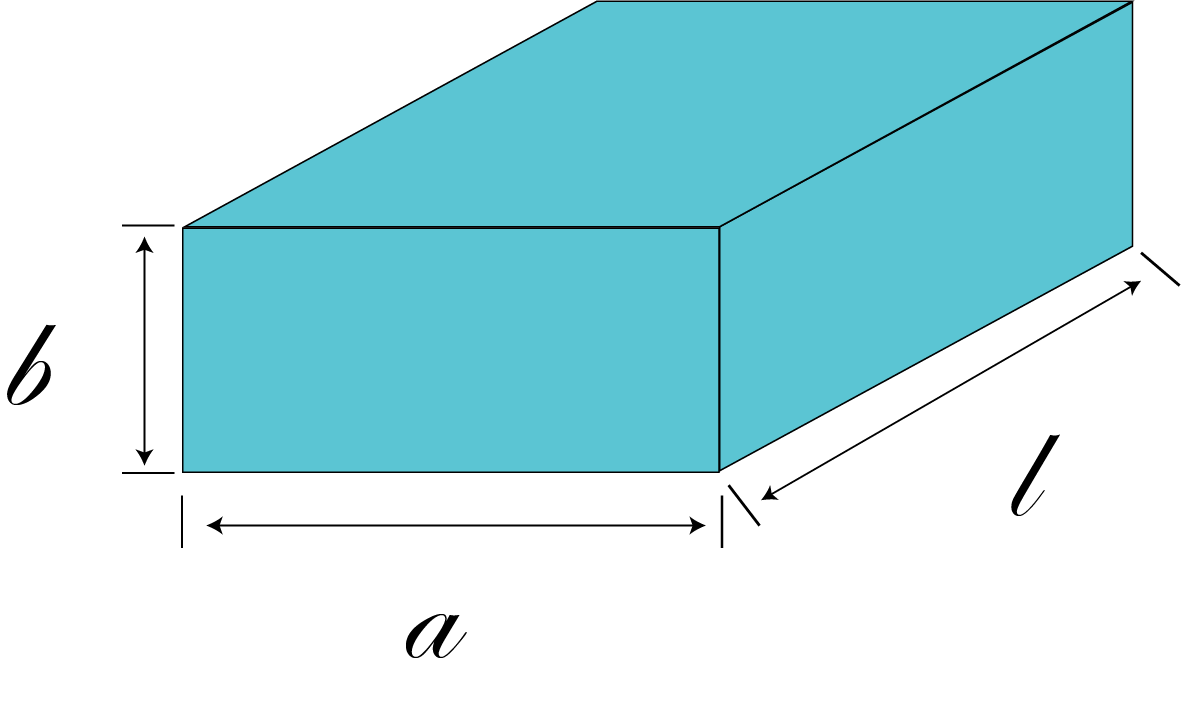
\includegraphics[width=8cm]{./image/空洞共振器.png}
    \caption{方形空洞共振器}
    \label{fig:Cavity}
  \end{center}
\end{figure}

\[
 \frac{1}{\lambda} = (\frac{m}{2a})^2 + (\frac{n}{2b})^2 + (\frac{p}{2l})^2
\]

\subsection{空洞量子電磁力学実験}
共振器内に単一原子を置き、内部の原子と電場の間の電気双極子結合を利用して、単一量子システムを制御する物理をC-QED($cavity - Quantum ElectroDynamics$)と呼ぶ。

今回は光子→マイクロ波(共振器内の1モード)、原子→人口原子(ジョセフソン素子)に置き換えて特性を調べる実験を行う。超伝導回路を用いたc-QED実験はその性質から、curcuit-QEDとも呼ばれる。
